\documentclass[output=paper,
colorlinks,
citecolor=brown,
newtxmath
]{langscibook} 
\bibliography{localbibliography}
\usepackage{comment}
\usepackage{verbatimbox}

\newenvironment{fullgreenverb}
{\verbbox}
{\endverbbox\par\colorbox[RGB]{204,255,204}{\parbox{\textwidth}{\theverbbox}}\par}

\newenvironment{fullblueverb}
{\verbbox}
{\endverbbox\par\colorbox[RGB]{204,229,255}{\parbox{\textwidth}{\theverbbox}}\par}
\newenvironment{fullgrayverb}
{\verbbox}
{\endverbbox\par\colorbox[RGB]{211,211,211}{\parbox{\textwidth}{\theverbbox}}\par}


\author{Steve Harris, Garlik, a part of Experian
Andy Seaborne, The Apache Software Foundation\affiliation{W3C}}
\title{SPARQL Presentation}  
\abstract{RDF is a directed, labeled graph data format for representing information in the Web.
SPARQL can be used to express queries across diverse data sources, whether the data is stored natively as RDF or reviewed as RDF via middleware. The results of SPARQL queries can be result sets or RDF graphs.
}

% add all extra packages you need to load to this file  
\usepackage{tabularx} 

%%%%%%%%%%%%%%%%%%%%%%%%%%%%%%%%%%%%%%%%%%%%%%%%%%%%
%%%                                              %%%
%%%           Examples                           %%%
%%%                                              %%%
%%%%%%%%%%%%%%%%%%%%%%%%%%%%%%%%%%%%%%%%%%%%%%%%%%%% 
%% to add additional information to the right of examples, uncomment the following line
% \usepackage{jambox}
%% if you want the source line of examples to be in italics, uncomment the following line
% \renewcommand{\exfont}{\itshape}
% \usepackage{./langsci/styles/jambox}
\usepackage{./langsci/styles/langsci-lgr}
\usepackage{./langsci/styles/langsci-osl}
\usepackage{langsci-optional}
\usepackage{langsci-gb4e}
\usepackage{langsci-cgloss}

\usepackage[linguistics]{forest}
\makeatletter
\let\thetitle\@title
\let\theauthor\@author 
\makeatother

\newcommand{\togglepaper}[1][0]{ 
%   \bibliography{../localbibliography}
  \papernote{\scriptsize\normalfont
    \theauthor.
    \thetitle. 
    To appear in: 
    Change Volume Editor \& in localcommands.tex 
    Change volume title in localcommands.tex
    Berlin: Language Science Press. [preliminary page numbering]
  }
  \pagenumbering{roman}
  \setcounter{chapter}{#1}
  \addtocounter{chapter}{-1}
}

% \IfFileExists{../localcommands.tex}{%hack to check whether this is being compiled as part of a collection or standalone
%   % add all extra packages you need to load to this file  
\usepackage{tabularx} 

%%%%%%%%%%%%%%%%%%%%%%%%%%%%%%%%%%%%%%%%%%%%%%%%%%%%
%%%                                              %%%
%%%           Examples                           %%%
%%%                                              %%%
%%%%%%%%%%%%%%%%%%%%%%%%%%%%%%%%%%%%%%%%%%%%%%%%%%%% 
%% to add additional information to the right of examples, uncomment the following line
% \usepackage{jambox}
%% if you want the source line of examples to be in italics, uncomment the following line
% \renewcommand{\exfont}{\itshape}
% \usepackage{./langsci/styles/jambox}
\usepackage{./langsci/styles/langsci-lgr}
\usepackage{./langsci/styles/langsci-osl}
\usepackage{langsci-optional}
\usepackage{langsci-gb4e}
\usepackage{langsci-cgloss}

\usepackage[linguistics]{forest}
%   \makeatletter
\let\thetitle\@title
\let\theauthor\@author 
\makeatother

\newcommand{\togglepaper}[1][0]{ 
%   \bibliography{../localbibliography}
  \papernote{\scriptsize\normalfont
    \theauthor.
    \thetitle. 
    To appear in: 
    Change Volume Editor \& in localcommands.tex 
    Change volume title in localcommands.tex
    Berlin: Language Science Press. [preliminary page numbering]
  }
  \pagenumbering{roman}
  \setcounter{chapter}{#1}
  \addtocounter{chapter}{-1}
} 
%\togglepaper[23]
% }{}

\begin{document}
\maketitle

% The part below is from the generic LangSci Press template for papers in edited volumes. Delete it when you're ready to go.

\section{Introduction} 
RDF is a directed, labeled graph data format for representing information in the Web. RDF is often used to represent, among other things; personal information, social networks, metadata about digital artifacts, as well as to provide a means of integration over disparate sources of information.
\subsection{Document Conventions}
\subsubsection{Namespaces}
In this document, examples assume the following namespace prefix bindings unless otherwise stated:

\begin{figure}[htp]\centering
\caption{name space binding}
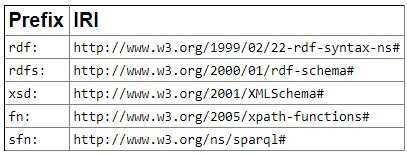
\includegraphics{langsci/img/namespacePrefixBindings.jpg}
\end{figure}

\subsubsection{Terminology}
The SPARQL language includes IRIs. IRIs include URIs and URLs.



\section{Making Simple Queries}
\subsection{Matching RDF Literals}
\label{fig:rdf literal example} shows an example of the data graph 
\begin{figure}[htp]\centering
\caption{matching RDF literal example}
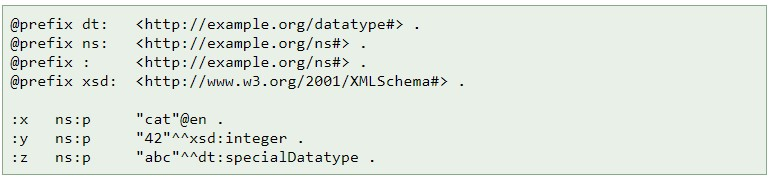
\includegraphics[scale=0.8]{langsci/img/rdfLiteralExample.jpg}
\label{fig:rdf literal example}
\end{figure} 
\subsubsection{Matching Literals with Language Tags}
Language tags in SPARQL are expressed using @ and the language tag.
This following query has no solution because "cat" is not the same RDF literal as "cat"@en:
\begin{verbatim}
SELECT ?x WHERE {?v ?p "cat"}
\end{verbatim}
but the query below will find a solution where variable is bound to :x because the language tag is specified and matches the givend data:
\begin{verbatim}
SELECT ?v WHERE {?v ?p "cat"@en}
\end{verbatim}
the result is:
\begin{verbatim}
 v
 <http://example.org/ns#x>
\end{verbatim}

\subsubsection{Matching Literals with Numeric Types}
Integers in a SPARQL query indicate an RDF typed literal with the datatype xsd:integer. For exmple: 42 is a shorteded form of 
\begin{verbatim}
"42"^^<http://www.w3.org/2001/XMLSchema#integer>
\end{verbatim}
\subsection{Creating Values With Expessions}
SparQL 1.1 allows to create values from complex expressions. The queries below show how to the \textcolor{blue}{CONCAT} function can be used to concatenate first names and last names from foaf data, then assign the value usig an \textcolor{blue}{expression in the SELECT clause} and also assign the value by using the \textcolor{blue}{BIND} form.
Data:
\begin{fullgreenverb}
@prefix foaf:  <http://xmlns.com/foaf/0.1/> .
      
_:a  foaf:givenName   "John" .
_:a  foaf:surname  "Doe" .
\end{fullgreenverb}

Query:
\begin{fullblueverb}
PREFIX foaf:   <http://xmlns.com/foaf/0.1/>
SELECT ( CONCAT(?G, " ", ?S) AS ?name )
WHERE  { ?P foaf:givenName ?G ; foaf:surname ?S }
\end{fullblueverb}

Query:
\begin{fullblueverb}
PREFIX foaf:   <http://xmlns.com/foaf/0.1/>
SELECT ?name
WHERE  { 
  ?P foaf:givenName ?G ; 
     foaf:surname ?S 
BIND(CONCAT(?G, " ", ?S) AS ?name)
}
\end{fullblueverb}
And then the result for those two queries are the same:
\begin{fullgrayverb}
name
"John Doe"
\end{fullgrayverb}



\newenvironment{fullgreenverb}
{\verbbox}
{\endverbbox\par\colorbox[RGB]{204,255,204}{\parbox{\textwidth}{\theverbbox}}\par}

\newenvironment{fullblueverb}
{\verbbox}
{\endverbbox\par\colorbox[RGB]{204,229,255}{\parbox{\textwidth}{\theverbbox}}\par}
\newenvironment{fullgrayverb}
{\verbbox}
{\endverbbox\par\colorbox[RGB]{211,211,211}{\parbox{\textwidth}{\theverbbox}}\par}

\section{RDF Term Constraints}
Graph pattern matching produces a solution sequence, where each solution has a set of binding of variables to RDF terms. SPARQL \textbf{FILTER} restrict solutions o those for which the filter expression evaluates to \textbf{TRUE}
We will introduce this section using the daa graph below:
\begin{fullgreenverb}
@prefix dc:   <http://purl.org/dc/elements/1.1/> .
@prefix :     <http://example.org/book/> .
@prefix ns:   <http://example.org/ns#> .

:book1  dc:title  "SPARQL Tutorial" .
:book1  ns:price  42 .
:book2  dc:title  "The Semantic Web" .
:book2  ns:price  23 .
\end{fullgreenverb}
\subsection{Restricting the Value of Strings}
SPARQL \textbf{FILTER} functions like \textcolor{blue}{regex} can test RDF literals. \textbf{regex} matches only strig literals, \textbf{regex} ca be used to match the lexical forms of other literals by using the str function.
Query:
\begin{fullblueverb}
PREFIX  dc:  <http://purl.org/dc/elements/1.1/>
SELECT  ?title
WHERE   { ?x dc:title ?title
          FILTER regex(?title, "^SPARQL") 
        }
\end{fullblueverb}
This query will return the title which begins with "SPARQL".
Query Result:
\begin{fullgrayverb}
"SPARQL Tutorial"
\end{fullgrayverb}
Regular expression matches may be made case-insensitive with the "i" flag.
Query:
\begin{fullblueverb}
PREFIX  dc:  <http://purl.org/dc/elements/1.1/>
SELECT  ?title
WHERE   { ?x dc:title ?title
          FILTER regex(?title, "web", "i" ) 
        }
\end{fullblueverb}
This query will return the title containing the "web", "web" can be minuscule or uppercase.
Query Result:
\begin{fullgrayverb}
title
"The Semantic Web"
\end{fullgrayverb}


\newenvironment{fullgreenverb}
{\verbbox}
{\endverbbox\par\colorbox[RGB]{204,255,204}{\parbox{\textwidth}{\theverbbox}}\par}

\newenvironment{fullblueverb}
{\verbbox}
{\endverbbox\par\colorbox[RGB]{204,229,255}{\parbox{\textwidth}{\theverbbox}}\par}
\newenvironment{fullgrayverb}
{\verbbox}
{\endverbbox\par\colorbox[RGB]{211,211,211}{\parbox{\textwidth}{\theverbbox}}\par}

\section{SPARQL Syntax}
\subsection{RDF Term Syntax}
\subsubsection{Syntax for Query Variables}
A query variable is marked by the use of either "?" or "\$"; the "?" or "\$" is not part of the variable name. In a query, \$abc and ?abc identify the same variable.
\subsubsection{Synax for Blank Nodes}
\begin{fullblueverb}
[ :p "v" ] .
[] :p "v" .
\end{fullblueverb}
they have allocated a unique blank node label (here "b57") and are equivalent to:
\begin{fullblueverb}
_:b57 :p "v" .
\end{fullblueverb}
When two triple patterns have the same subject:
\begin{fullblueverb}
[ :p "v" ] :q "w" .
\end{fullblueverb}
which is equivelent to:
\begin{fullblueverb}
_:b57 :p "v" .
_:b57 :q "w" .
\end{fullblueverb}
When they have the same object:
\begin{fullblueverb}
:x :q [ :p "v" ] .
\end{fullblueverb}
which is equivelent to:
\begin{fullblueverb}
:x  :q _:b57 .
_:b57 :p "v" .
\end{fullblueverb}
\subsubsection{RDF Collections}
RDF collections can be written in triple patterns using the syntax "(element1 element2 ...)". The form "()" is an alternative for the IRI http://www.w3.org/1999/02/22-rdf-syntax-ns#nil. When used with collection elements, such as (1 ?x 3 4), triple patterns with blank nodes are allocated for the collection. \textbf{The blank node at the head of the collection can be used as a subject or object in other triple patterns}. The blank nodes allocated by the collection syntax do not occur elsewhere in the query.
\begin{fullblueverb}
(1 ?x 3 4) :p "w" .
\end{fullblueverb}
is syntactic sugar for:
\begin{fullblueverb}
 _:b0  rdf:first  1 ;
          rdf:rest   _:b1 .
_:b1  rdf:first  ?x ;
          rdf:rest   _:b2 .
_:b2  rdf:first  3 ;
      rdf:rest   _:b3 .
_:b3  rdf:first  4 ;
      rdf:rest   rdf:nil .
_:b0  :p         "w" .
\end{fullblueverb}
RDF collections can be nested and can involve other syntactic forms:
\begin{fullblueverb}
(1 [:p :q] ( 2 ) ) .
\end{fullblueverb}
is syntactc sugar for:
\begin{fullblueverb}
_:b0  rdf:first  1 ;
    rdf:rest   _:b1 .
_:b1  rdf:first  _:b2 .
_:b2  :p         :q .
_:b1  rdf:rest   _:b3 .
_:b3  rdf:first  _:b4 .
_:b4  rdf:first  2 ;
      rdf:rest   rdf:nil .
_:b3  rdf:rest   rdf:nil .
\end{fullblueverb}
\subsubsection{rdf:type}
The keywrd "a" ca be used as a predicate in a riple pattern and is an alternative for \textcolor{blue}{http://www.w3.org/1999/02/22-rdf-syntax-ns#type}. This keyword is case-sensitive.
\begin{fullblueverb}
?x  a  :Class1 .
[ a :appClass ] :p "v" .
\end{fullblueverb}
is syntactic sugar for:
\begin{fullblueverb}
?x    rdf:type  :Class1 .
_:b0  rdf:type  :appClass .
_:b0  :p        "v" .
\end{fullblueverb}

\newenvironment{fullgreenverb}
{\verbbox}
{\endverbbox\par\colorbox[RGB]{204,255,204}{\parbox{\textwidth}{\theverbbox}}\par}

\newenvironment{fullblueverb}
{\verbbox}
{\endverbbox\par\colorbox[RGB]{204,229,255}{\parbox{\textwidth}{\theverbbox}}\par}
\newenvironment{fullgrayverb}
{\verbbox}
{\endverbbox\par\colorbox[RGB]{211,211,211}{\parbox{\textwidth}{\theverbbox}}\par}

\section{Negation}
\subsection{Difference between Not Exists and Minus}
In order to explain the difference, here we give the data graph as the following:
\begin{fullgreenverb}
@prefix : <http://example.com/> .
:a :p 1 .
:a :q 1 .
:a :q 2 .

:b :p 3.0 .
:b :q 4.0 .
:b :q 5.0 .
\end{fullgreenverb}
At this moment, if we use the \textcolor{blue}{NOT EXISTS} query like the following:
\begin{fullblueverb}
PREFIX : <http://example.com/>
SELECT * WHERE {
        ?x :p ?n
        FILTER NOT EXISTS {
                ?x :q ?m .
                FILTER(?n = ?m)
        }
}
\end{fullblueverb}
then we have the results
\begin{fullgrayverb}
x                           n
<http://example.com/b>      3.0
\end{fullgrayverb}
Whereas with \textcolor{blue}{MINUS}, like following:
\begin{fullblueverb}
PREFIX : <http://example/>
SELECT * WHERE {
        ?x :p ?n
        MINUS {
                ?x :q ?m .
                FILTER(?n = ?m)
        }
}
\end{fullblueverb}
We have the result
\begin{fullgrayverb}
x                           n
<http://example.com/b>      3.0
<http://example.com/a>	    1
\end{fullgrayverb}
because in the queries of \textcolor{blue}{MINUS}, there is no relation between the variables in the SELECT clause and in the MINUS clause, so we do not know what does ?n represent. However, in the NOT EXISTS clause, the variable ?n in NOT EXISTS clause is bounded to the ?n in the SELECT clause.
\section{Property Paths}
\subsection{Arbitrary Length Path Matching}
Connectivity between the subject and object by a property path of arbitrary length can be found using the "zero or  more" property path operator, "*", and the "one or more" property path operator , +. There is also "zeros or one" connectivity property path operator, ?.
all of these quantities express the existence number of this property which has these operators.
for example, in the query below:
\begin{fullblueverb}
PREFIX foaf: <http://xmlns.com/foaf/0.1/>
PREFIX :     <http://example/>
SELECT ?person
{ 
    :x foaf:knows+ ?person
}
\end{fullblueverb}
it means that find all the persons that x knows. In this case, foaf:know can be used multiple times to find the answer.




\end{document}
